\chapter{Methods}
\label{c:methods}

\section{Inspection Platform Structure}
Refer to Kumar's work \cite{kumar2008computer}, we designed a scalable platform could install multiple cameras. Use one PC as host machine to collect images from camera array.
After retrieved images from camera, the defect detection methods (Lettering Defect Detection \& LED Color inspection) described below will inspect wheather the keyboard has any defect on it. 
\begin{figure}
	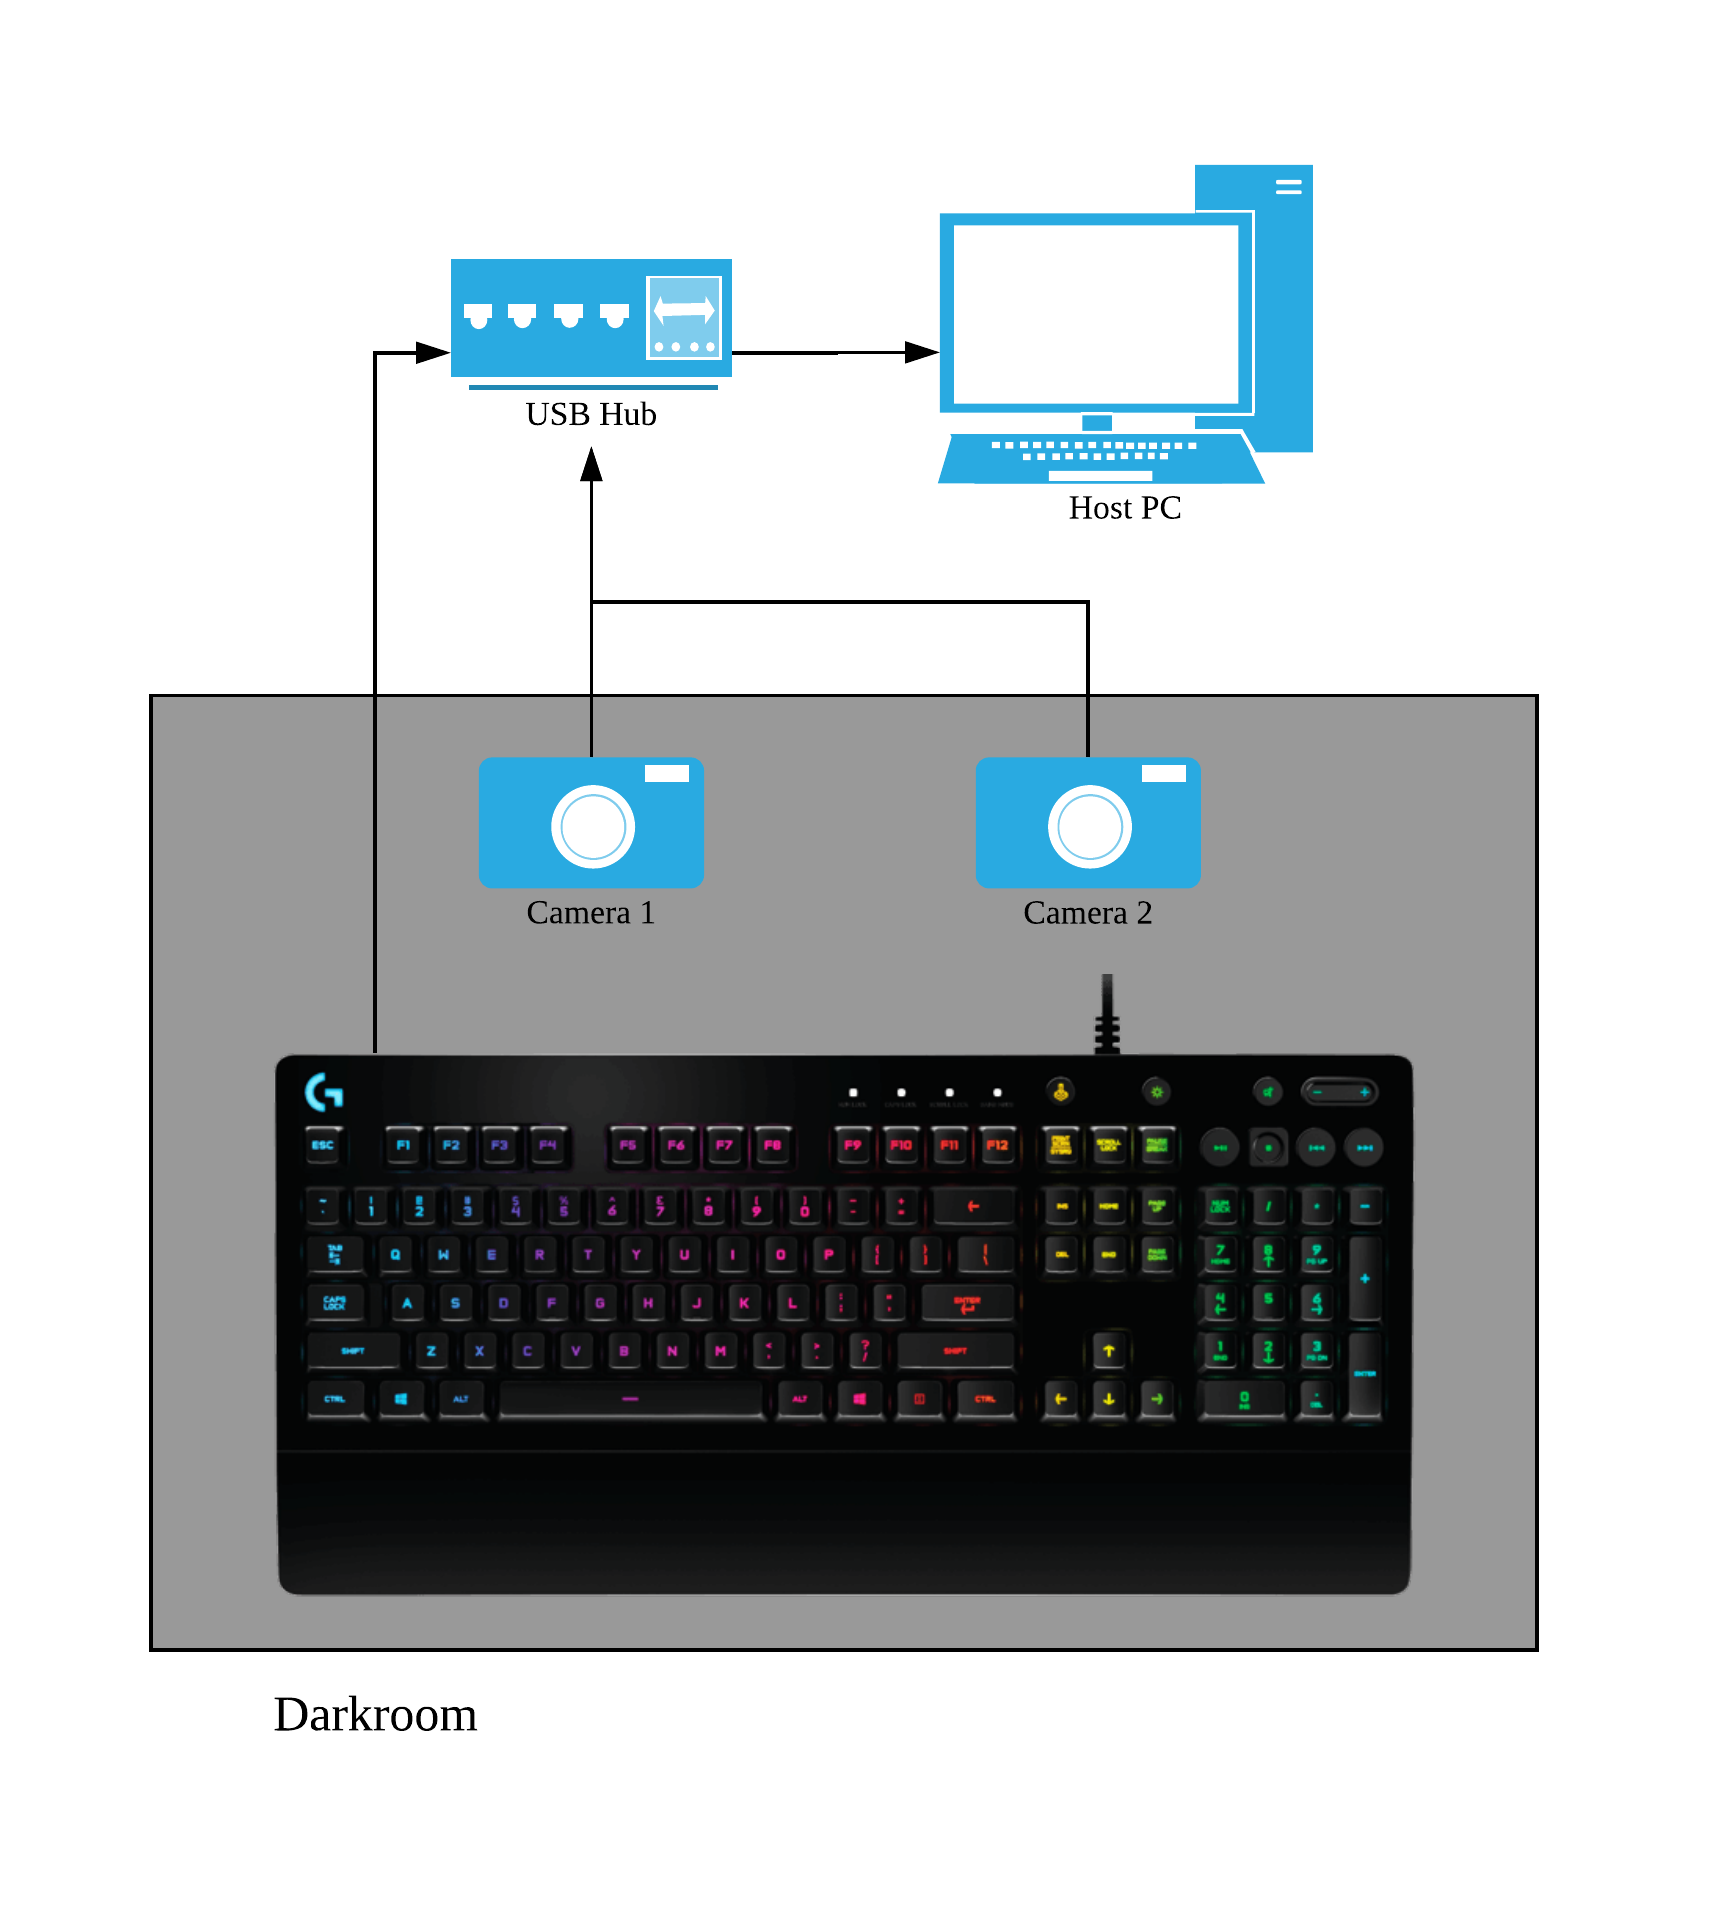
\includegraphics[width=\linewidth]{SystemStructure.png}
	\caption{The Diagram of SystemStructure}
	\label{fig:SystemStructure}
\end{figure}


\section{Lettering Defect Detection Intorduction}
\label{letteringDetection}
	In lettering defect detection, we want to check the layout of keyboard and quality of laser engraving on each key.
	We'll give a detailed explan of how the lettering defect detection is designed and how they work.

	\subsection{Learning Stage} 
		Lettering defect detection can be saperated into two main part.
		The first part is learning stage. This part reads the gold image from file and doing the feature point detection, and store the feature points \& their descriptor for examining stage use.

		\begin{figure}
			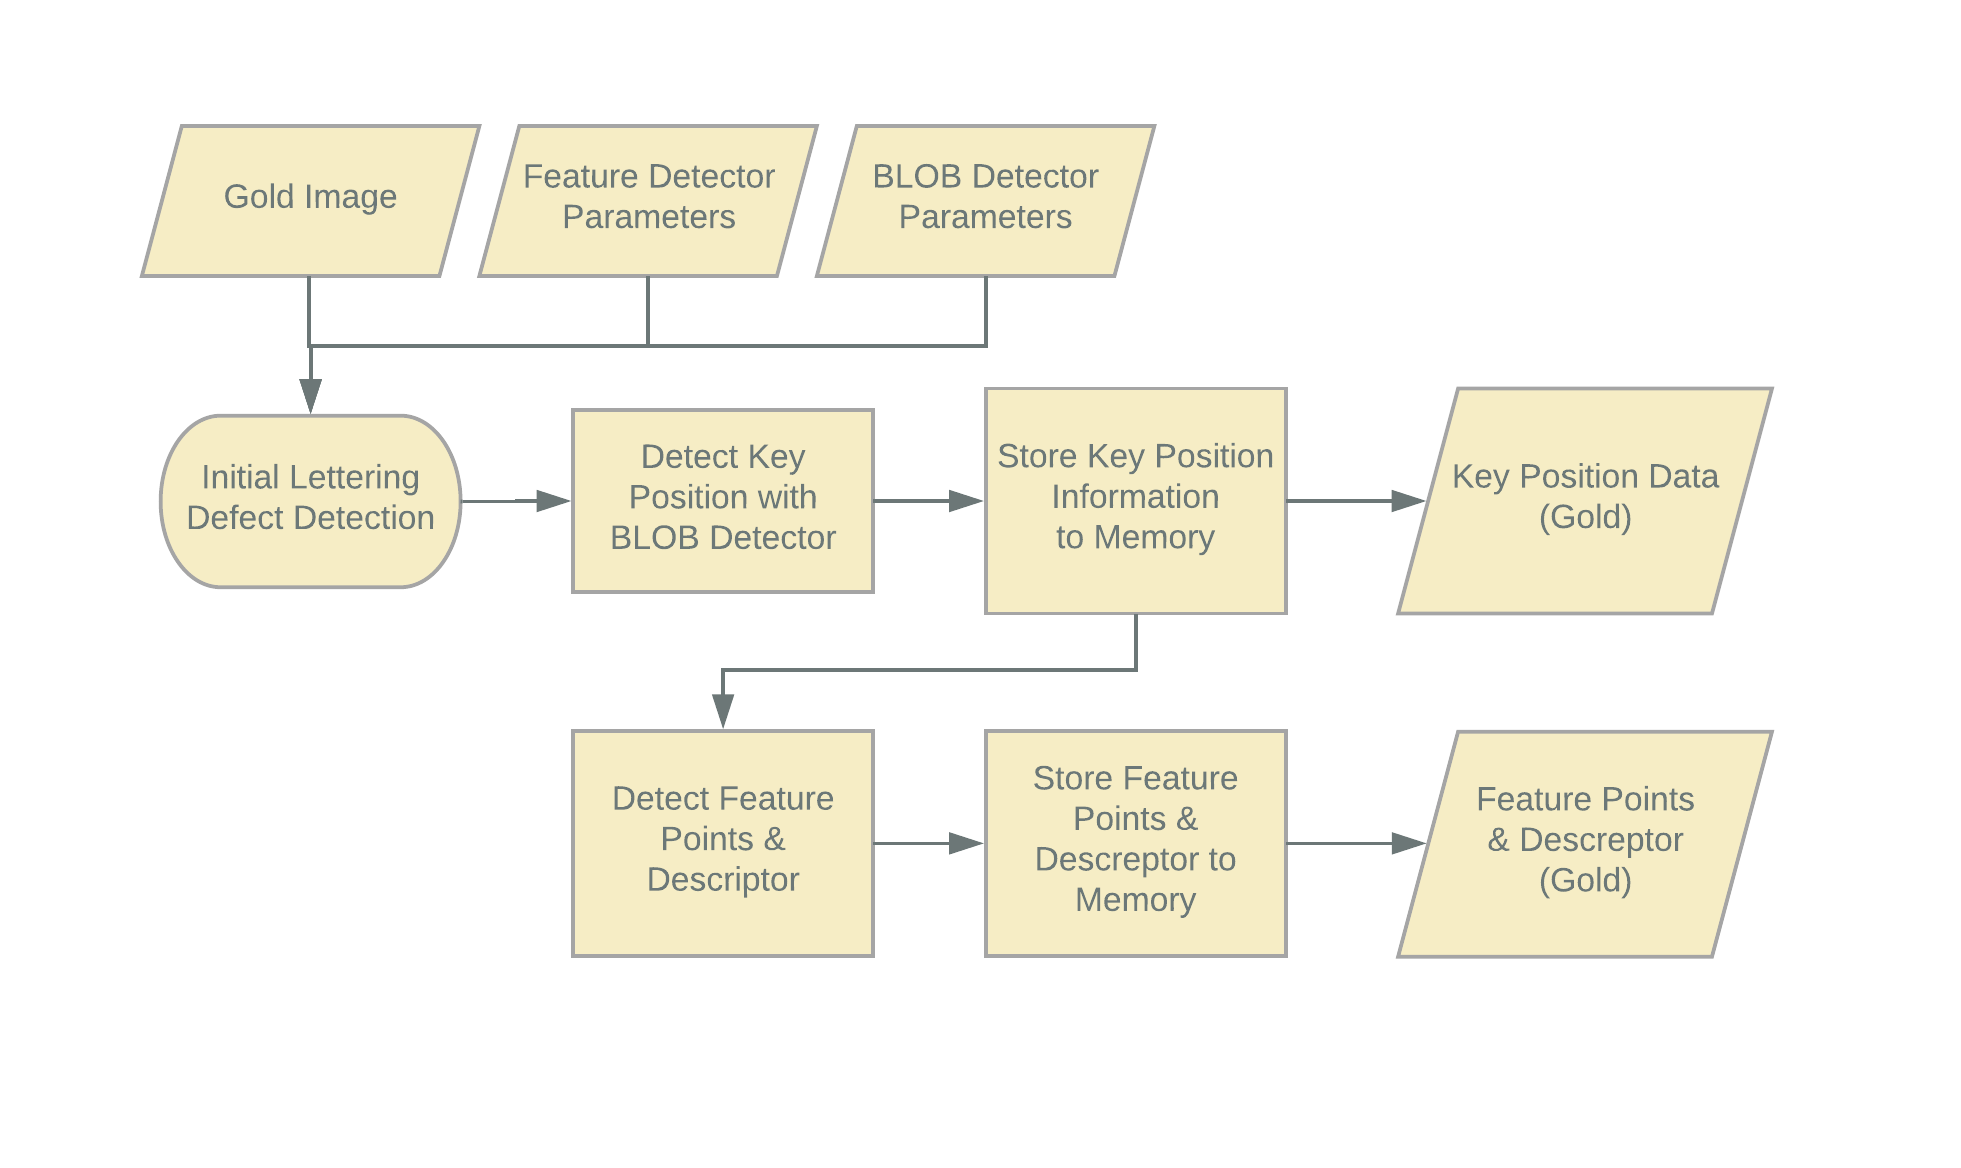
\includegraphics[width=\linewidth]{LetteringInit.png}
			\caption{The Diagram of Lettering Initialize Stage}
			\label{fig:LetteringInit}
		\end{figure}

	\subsection{Inspection Stage}
		In lattering examing stage, we did same steps on the keyboard sample image we want to imspect, doing the feature point detection and store the feature points \& their descriptor.
		After having the feature point and descriptor from both gold \& keyboard sample image, we do the feature point matching to find the homography matrix then we can align sample image with gold image with geomatric transformantion. 
		With both image aligned, we apply the defect detection method to aligned images, and get the marked defect information.
		And judge the sample keyboard is a defected on or a good one.
		\begin{figure}
			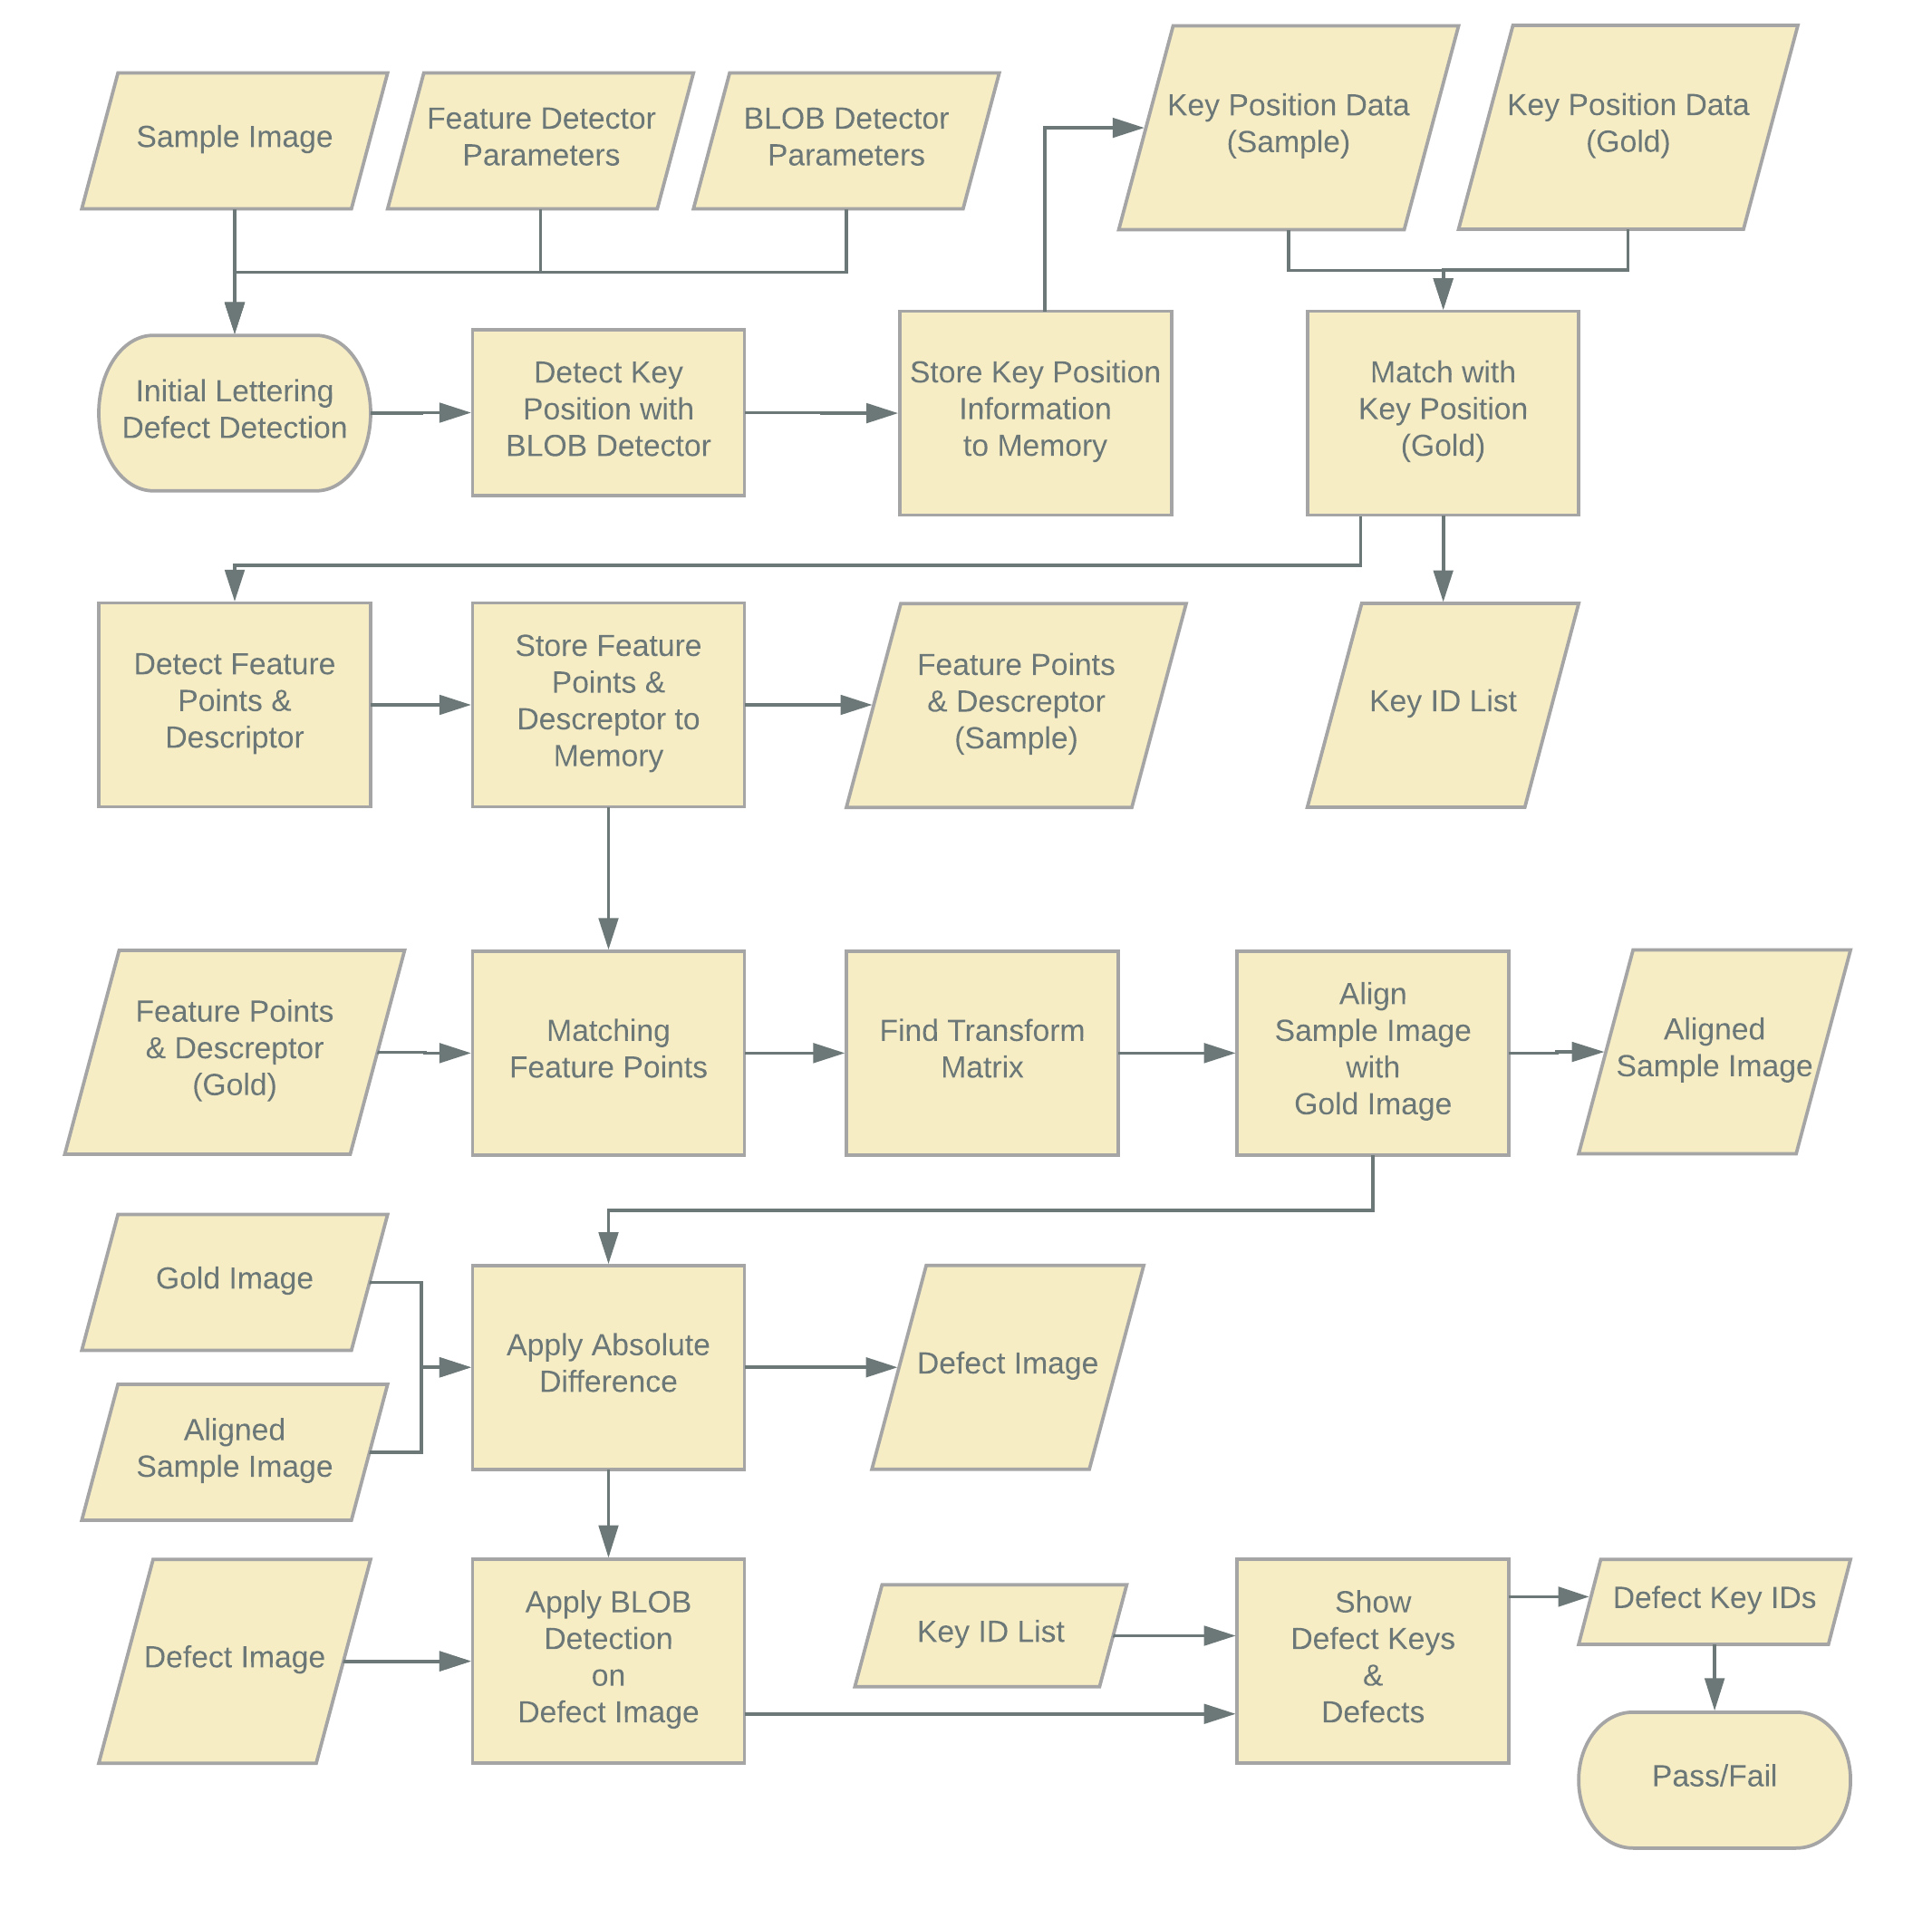
\includegraphics[width=\linewidth]{LetteringInspection.png}
			\caption{The Diagram of Lettering Inspection Stage}
			\label{fig:LetteringInspection}
		\end{figure}

	\subsection{Defect Detection Method}
		In lettering defect detection, after gray-scale gold \& smaple image aligned, we calculate absolute difference of two image, and get a new gray scale image, say $M_{Diff}$, that contained defects information.
		To detect the defect, we could apply simple blob detection with soutable parameters to identify wheather a bright spot is defect or noise.
		
		$$ \textrm{add a flow chart here} $$
		$$ \textrm{add example image of absdiff result after alignment} $$

\section{LED Mulfunction Detection Intorduction}
	In LED function inspection, we want to check if each LED embadded in the circuit of keyboard functions as expect.
	In this stage, we'll capture three pair of gold and sample image, $(gold_R, sample_R), (gold_G, sample_G), (gold_B, sample_B)$, used to inspect three different color chanel of LED light source.
	The detailed method will be described in following subsectinos.
	\subsection{Learning Stage}
		In this step, we want to build the pass standard with given gold image.
		By apply corresponding HSV filter, $filter_r, filter_g, filter_b$, to gold images, we can obtain three binary image, witch can use to identify if a testing object funcions as this binary image.
		\begin{figure}
			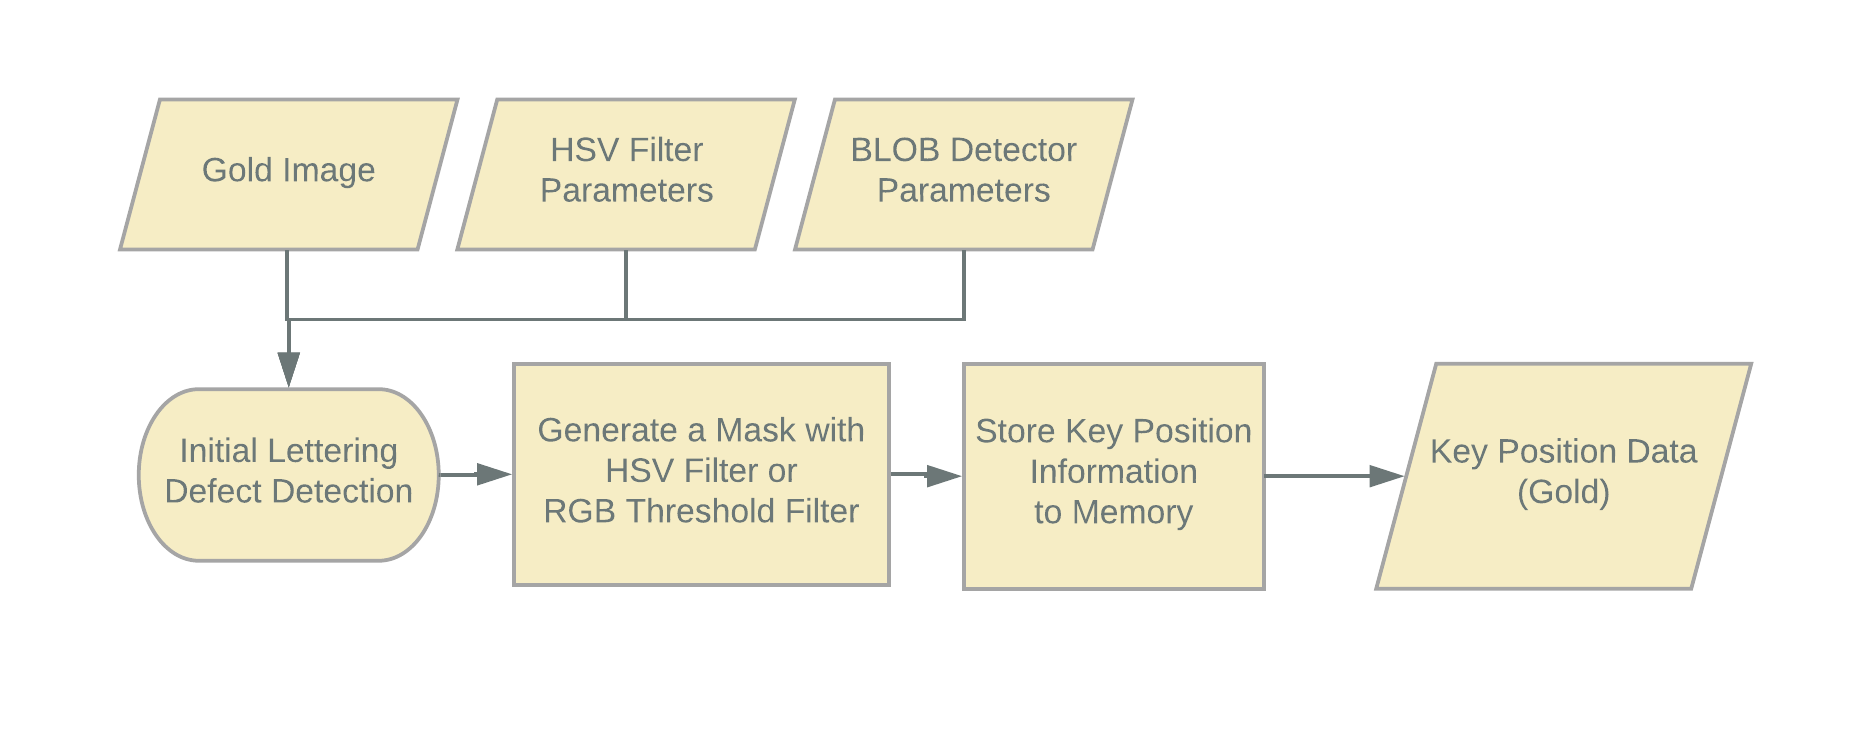
\includegraphics[width=\linewidth]{LEDInit.png}
			\caption{The Diagram of LED Initialize Stage}
			\label{fig:LEDInit}
		\end{figure}

	\subsection{Inspection Stage}
		In this step, we are going to check if a testing object functions as the passing standard.
		We applied same filter, say $filter_c$, on the image captured from camera. And get a binary image of testing object.
		We compare the blob size and shape between the binary image of gold and sample, to see if there is any mulfunctioning on the LED lights.
		\begin{figure}
			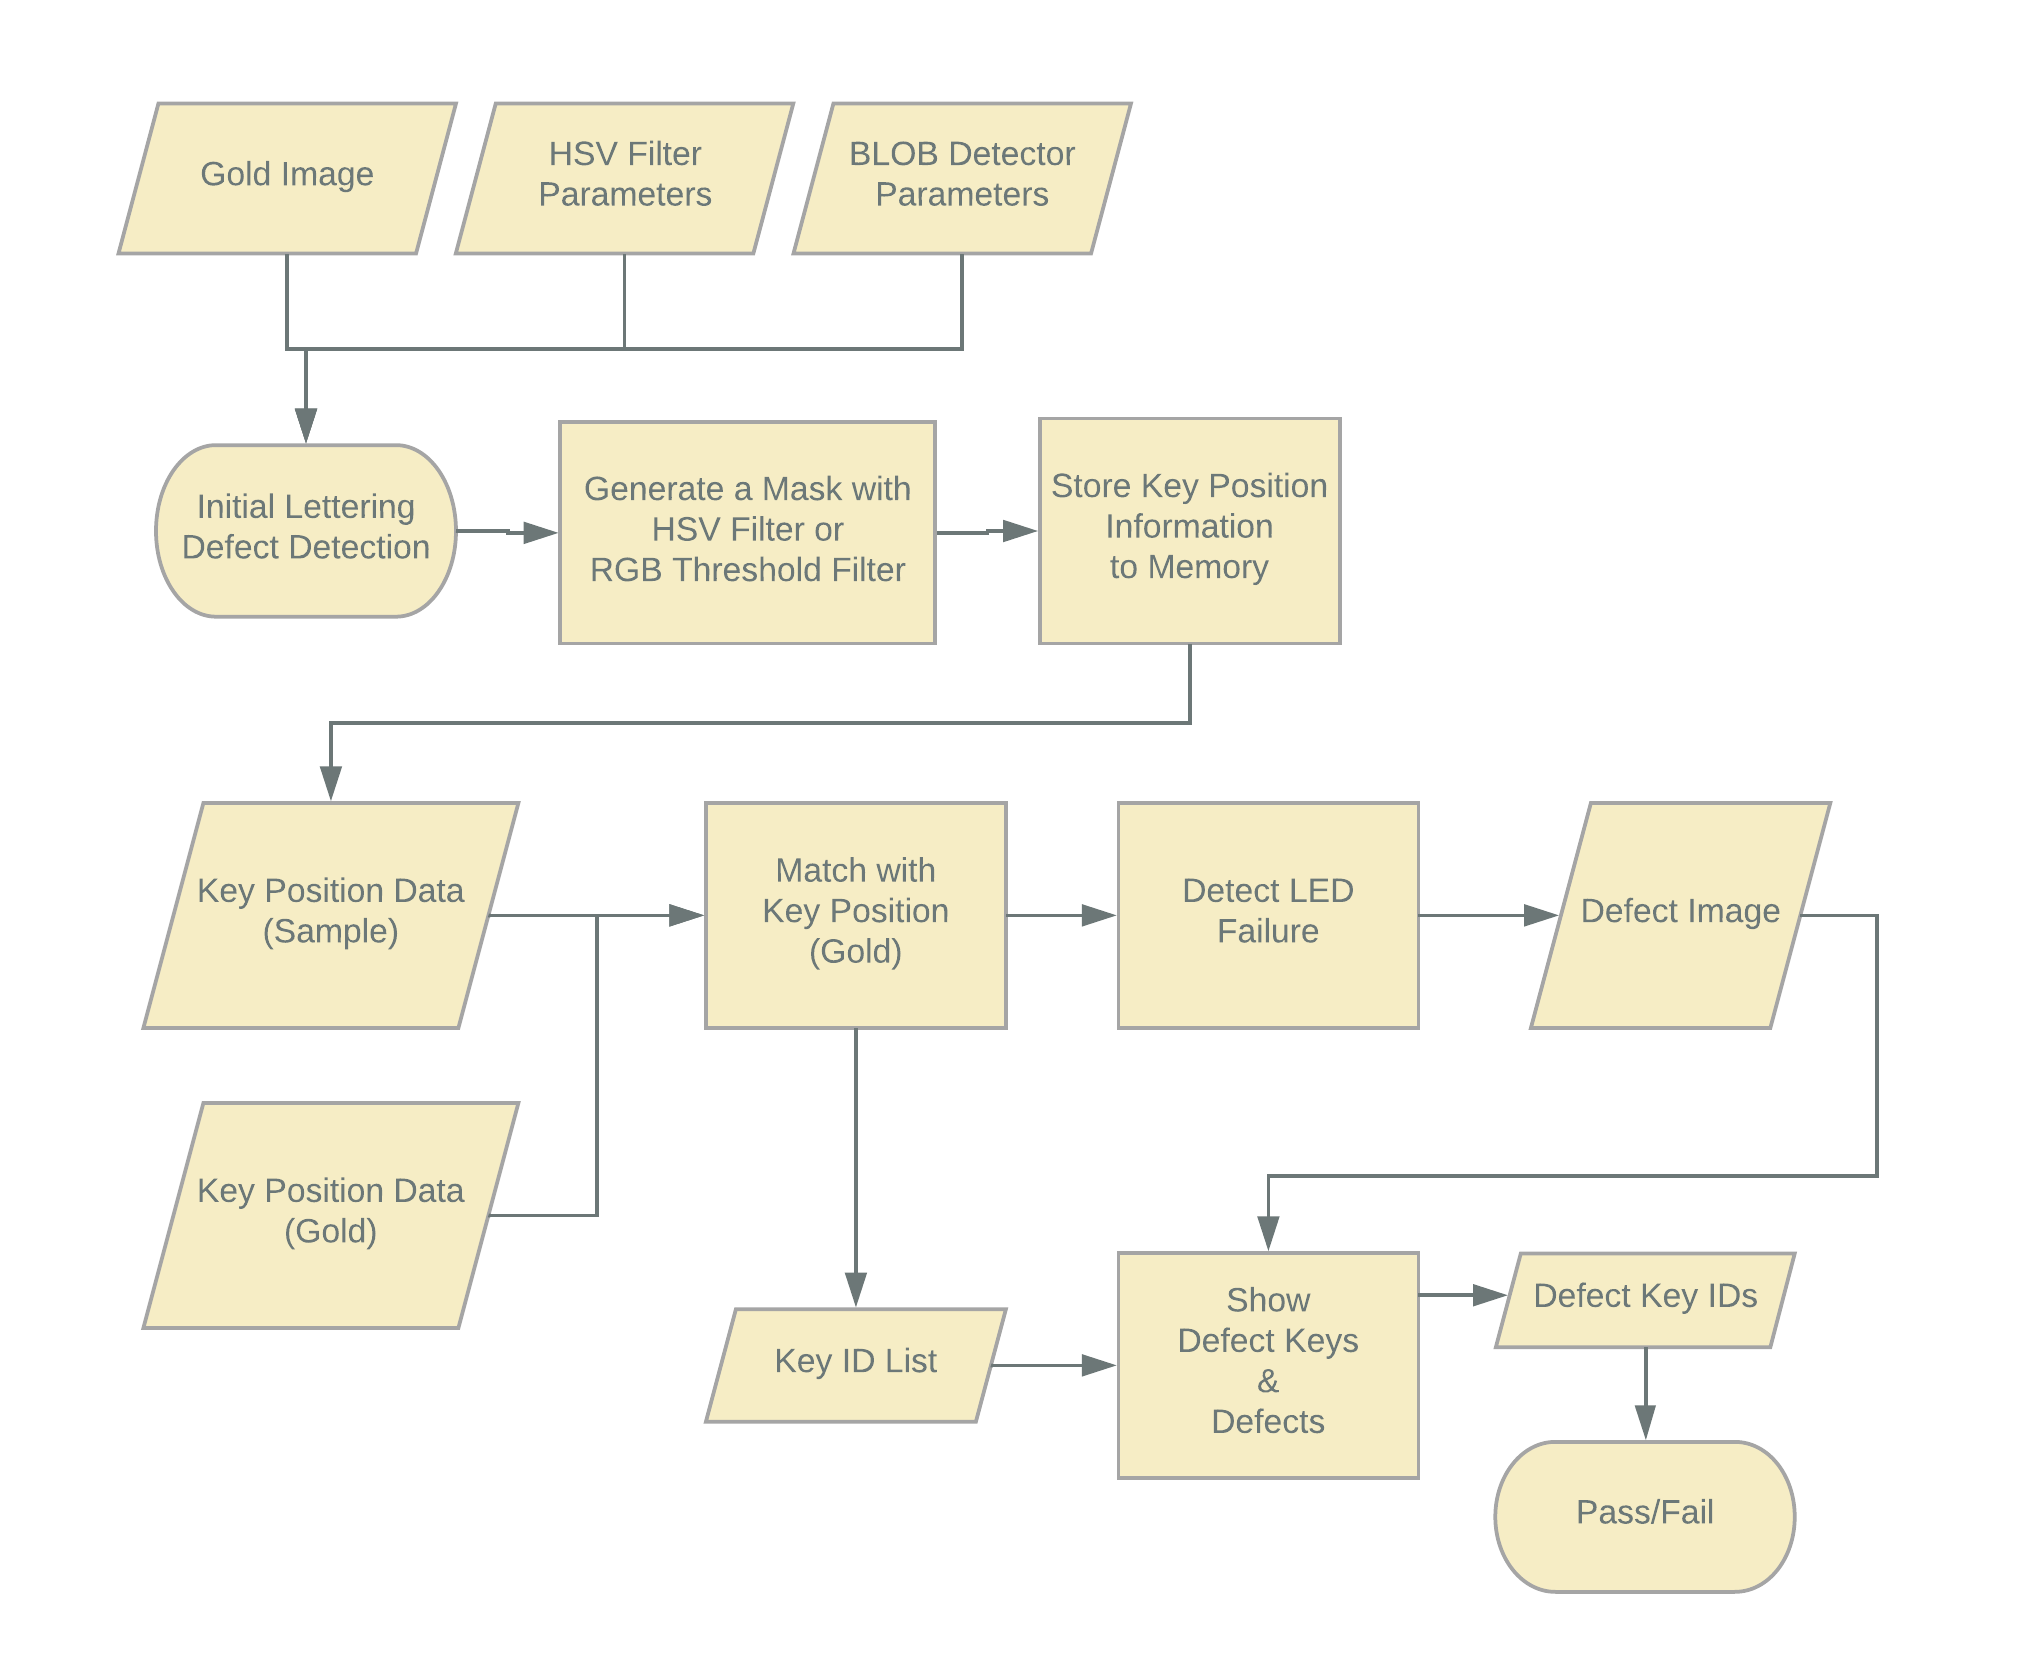
\includegraphics[width=\linewidth]{LEDInspection.png}
			\caption{The Diagram of LED Inspection Stage}
			\label{fig:LEDInspection}
		\end{figure}

\section{Other Functions Implemented}
	\subsection{Stamp Detection}
		Stamp detection is implemented after lattering defect detection is implemented.
		Since the steps doing object detection and feature based image alignment are very similar.
		We first applied feature point detect method on the stamp image and image that we want to inspect.
		After applied point matching methods, we could find the posible area for the stamp.
		Finally, we compare the similarity between the posible area, make sure that there is no misjudge on the inspection.